%(BEGIN_QUESTION)
% Copyright 2010, Tony R. Kuphaldt, released under the Creative Commons Attribution License (v 1.0)
% This means you may do almost anything with this work of mine, so long as you give me proper credit

Beregn vekten, forutsatt at påført lufttrykk akkurat er nok til å løfte den mot tyngdekraften. Anta et stempel med ytre diameter 12.5 tommer og stangdiameter 2.8 tommer:

$$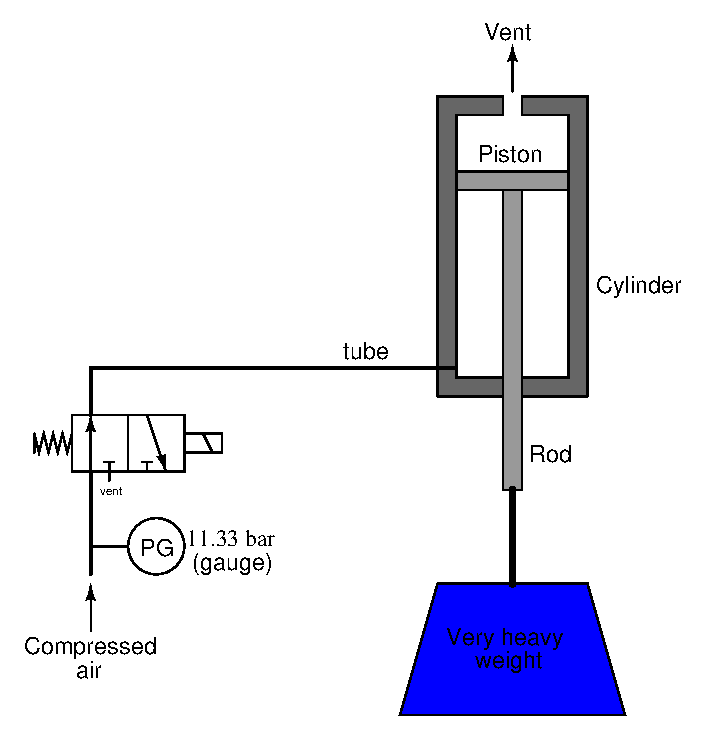
\includegraphics[width=15.5cm]{i01627x01.eps}$$

Vekt = \underbar{\hskip 50pt} lbs

\vskip 10pt

Angi også om magnetventilen må være {\it energisert} eller {\it av-energisert} for å løfte vekten.

\underbar{file i01627}
%(END_QUESTION)





%(BEGIN_ANSWER)

Jeg anbefaler å gi 7 poeng for korrekt svar på vekt, og 3 poeng for korrekt svar om magnetventilen:

\vskip 10pt

Vekt = \underbar{\bf 19,150 lbs}

\vskip 10pt

Magnetventilen må være {\bf av-energisert} for at sylinderen skal løfte vekten.

%(END_ANSWER)





%(BEGIN_NOTES)

{\bf Dette spørsmålet er kun ment for eksamen, ikke arbeidsark!}.

%(END_NOTES)
